%%%%%%%%%%%%%%%%%%%%%%%%%%%%%%%%%%%%%%%%%%%%%%%%%%%%%%%%%%%%%%%%%%%%%%%%%%%%%%%%
%2345678901234567890123456789012345678901234567890123456789012345678901234567890
%        1         2         3         4         5         6         7         8

\documentclass[letterpaper, 10 pt, conference]{ieeeconf}  % Comment this line out if you need a4paper

%\documentclass[a4paper, 10pt, conference]{ieeeconf}      % Use this line for a4 paper

\IEEEoverridecommandlockouts                              % This command is only needed if 
                                                          % you want to use the \thanks command

\overrideIEEEmargins                                      % Needed to meet printer requirements.

% See the \addtolength command later in the file to balance the column lengths
% on the last page of the document

% The following packages can be found on http:\\www.ctan.org
\usepackage{graphicx} % for pdf, bitmapped graphics files
\usepackage{epsfig} % for postscript graphics files
%\usepackage{mathptmx} % assumes new font selection scheme installed
%\usepackage{times} % assumes new font selection scheme installed
\usepackage{amsmath} % assumes amsmath package installed
\usepackage{amssymb}  % assumes amsmath package installed
\usepackage{algorithm}
\usepackage{algorithmic}

\usepackage{color}
\usepackage{bm} 
\usepackage{customCommands}

%\usepackage[pdflatex]{hyperref}

% More macros
\newcommand{\bw}{{\bfomega}}
\newcommand{\bth}{{\bftheta}}
\newcommand{\bphi}{{\bfphi}}
\newcommand{\nth}{\norm{\bth}}
\newcommand{\ab}{{\bfa_b}}
\newcommand{\wb}{{\bw_b}}
\newcommand{\D}{\Delta}
\newcommand{\Dzero}{{\D^0}}
\newcommand{\Dp}{{\D\bfp}}
\newcommand{\Dv}{{\D\bfv}}
\newcommand{\Dth}{{\D\bth}}
\newcommand{\Dq}{{\D\bfq}}
\newcommand{\DR}{{\D\bfR}}
\newcommand{\DP}{{\D\bfP}}
\newcommand{\DV}{{\D\bfV}}
\newcommand{\DTH}{{\D\bfTheta}}
\newcommand{\Dw}{{\D\bw}}
\newcommand{\DW}{{\D\bfOmega}}
\newcommand{\dpp}{{\delta\bfp}}
\newcommand{\dv}{{\delta\bfv}}
\newcommand{\dth}{{\delta\bth}}
\newcommand{\dq}{{\delta\bfq}}
\newcommand{\dR}{{\delta\bfR}}
\newcommand{\dP}{{\delta\bfP}}
\newcommand{\dV}{{\delta\bfV}}
\newcommand{\dTH}{{\delta\bfTheta}}
\newcommand{\dw}{{\delta\bw}}

\newcommand{\te}{\triangleq}
\newcommand{\od}{\odot}


%%%%%%%%%%%%%%%%%%%%%%%%%%%%%%%%%%%%%%%%%%%
\title{\LARGE \bf
Odometry Based on Auto-Calibrating Inertial Measurement Unit Attached to the Feet
}

\author{Dinesh Atchuthan$^{1}$, Angel Santamaria-Navarro$^{2}$, Nicolas Mansard$^1$, Olivier Stasse$^1$, Joan Sol\`a$^{1,2}$% <-this % stops a space
\thanks{$^{1}$ CNRS - LAAS, Toulouse, France, \tt {\footnotesize \{first.last\}@laas.fr}}%
\thanks{$^{2}$ IRI, UPC, Barcelona, \tt{\footnotesize \{asantamaria,jsola\}@iri.upc.edu}}
}

\begin{document}

\maketitle
\thispagestyle{empty}
\pagestyle{empty}

%%%%%%%%%%%%%%%%%%%%%%%%%%%%%%%%%%%%%%%%%%%%%%%%%%%%%%%%%%%%%%%%%%%%%%%%%%%%%%%%
\begin{abstract}
% !TEX root = main.tex
%
%
Location of pedestrian in indoor environment remains an open problem.
A cheap and reliable sensor in this context is the inertial measurement units (IMU), carried by the pedestrian while he/she is walking.
However, due to the bias of both the accelerometer and the gyroscope, integrating directly the inertial measurements leads to tremendous drift, as the state of the system (position, orientation, velocity, bias) is not fully observable. 
In this paper, we consider the specific case where an IMU is attached to one of the pedestrian's feet.
We exploit specific prior knowledges (i.e. the fact that the foot lands at zero velocity on a horizontal plane) in order to make the full state of the IMU observable.
The inertial measurements and these prior knowledges are gathered in a graphical model (a factor graph), and are exploited to build a maximum-likelihood estimator.
The technical difficulty is to handle the size of the graph such that it is tractable in a limited time window, that we do by relying on the pre-integration technique.
In that existing framework, our contributions are to reformulate the pre-integration method using quaternions while giving a simpler algebraic formulation, and to apply this method for estimating the human foot-pose during walking.
We validate these concepts on several long-range trajectories capture with human subject and compare the results with ground-truth measurements (coming from a motion capture system) and previous results of the state of the art.
%We show that our method is able to reconstruct its trajectory under some conditions.



%% In this paper, a graphical representation approach is presented to integrate 
%% IMU measurement on an augmented human. Although state estimators using both
%% informations \cite{Johnson:jof:2016,Fallon:ichr:2014} have been already proposed, this method has several additional interests.
%% First it is allowing to estimate bias and initial position of the IMU thanks to the graph
%% approach. Second the concept has been extensively used in the SLAM community and integrating 
%% other measurements such as laser, range image and so on can be done in a coherent mathematical framework.
%% The technical difficulty is to handle the size of the graph such that it is tractable in a limited window.
%% It was proposed in \cite{forster2015imu} to pre-integrate the most frequent data which are given by the IMU.
%% In this paper we propose a detailed derivation of this pre-integration using quaternion instead
%% of rotation matrices leading not only to faster computation and smaller memory foot-print,
%% but also to a more comprehensible pre-integration data to which we can give a physically coherent interpretation.
%% We validate these concepts by estimating the trajectory of the foot of a human agent during walking,
%% and show that we are able to reconstruct its trajectory under some conditions.

\end{abstract}


%%%%%%%%%%%%%%%%%%%%%%%%%%%%%%%%%%%%%%%%%%%%%%%%%%%%%%%%%%%%%%%%%%%%%%%%%%%%%%%%
% !TEX root = main.tex

\section{Introduction}\label{sec:intro}

One of the most common ways to describe the trajectory of a body in space is to use odometry, which can be derived from a multitude of sensors, from encoders to GPS and cameras.
The quality of this information is also known to be dependent on the sensor specifications and to accumulate measurement errors. 
The development of SLAM (Simultaneous Localization And Mapping) is mature enough to resolve 
this dependency over time with loop closure strategies. However, other strategies are required to comply with the particularities of legged locomotion and physical interactions in unstructured environments. 
This is particularly necessary in outdoor or industrial applications with cluttered environment. 
In this case, assuming a flat floor is not always reasonable and being able to observe the foot pose allows to implement advanced reactive locomotion strategies.

In the DRC \cite{Johnson:jof:2016,Marion:jof:2017,Karumanchi:jof:2017} most of the teams used laser or RGB-D cameras to build a reconstruction of the floor surface in order to \emph{plan}
the next feet pose. For some teams the level of accuracy was not always sufficient and involved dramatic failures despite intensive training \cite{Kaneko:ichr:2015}.
On the other hand, the IHMC team \cite{Johnson:jof:2016} reported an important gain in terms of accuracy using their state estimator alone,
reaching an impressive $1$\,cm drift per every three steps for the pelvis horizontal position,
and $5$\,mm per every nine steps for the pelvis vertical position. 
Using a quite simple state estimator, it is very interesting to note the following reported factors for reaching this level of precision besides bug fixing:
the redesign of Atlas, coming with a significant reduction of backlash in the leg joints, improving measurements using kinematics and a walking gait reducing the amount of foot slipping and bouncing.
Although the IHMC tested a localization algorithm \cite{Pomerlau:ar:2013}, occasional localization errors were a problem in the overall behavior and SLAM happened to be not necessary in this situation.

\begin{figure}
\centering
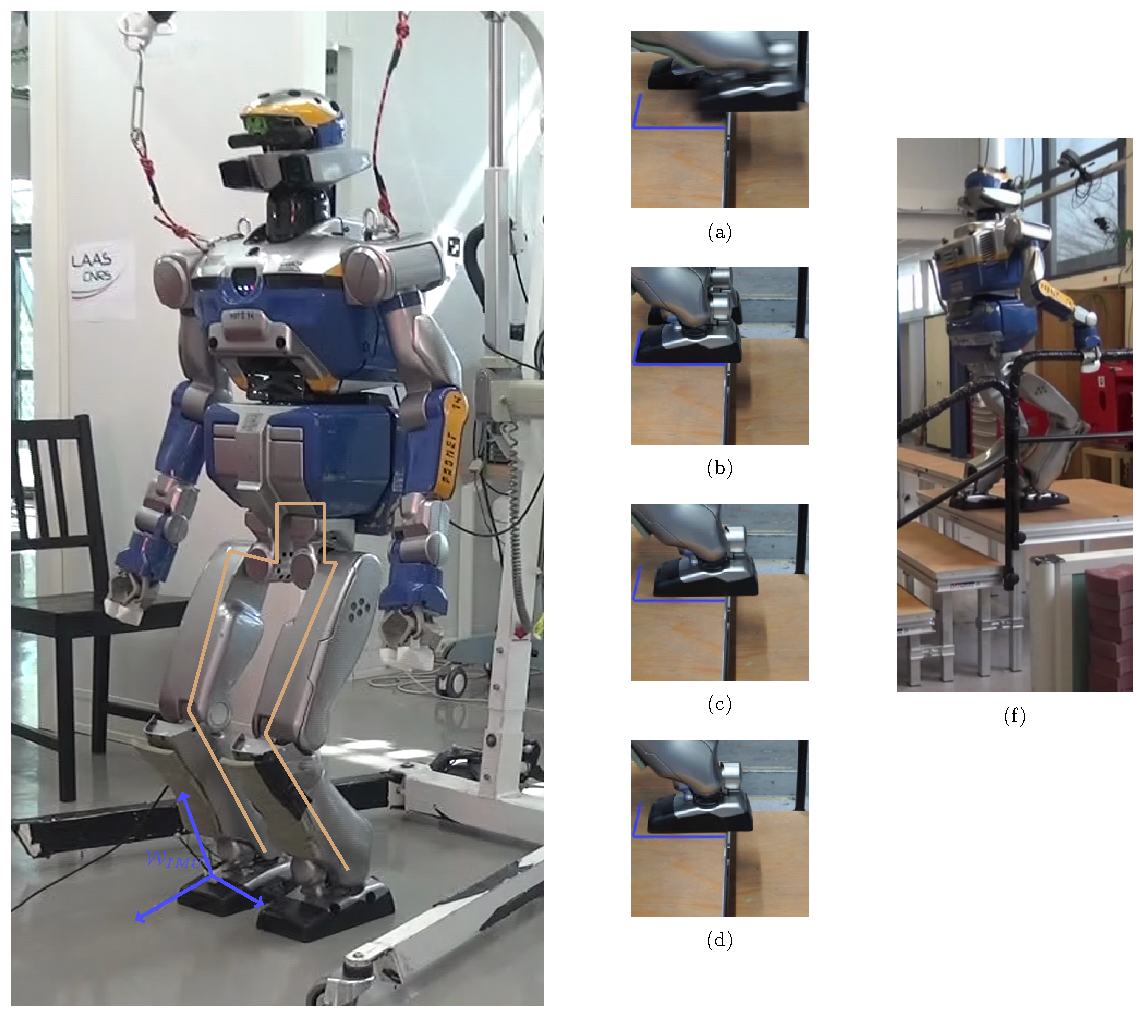
\includegraphics[width=\linewidth]{./figures/cover-figure.pdf}
	\caption{The flying foot trajectory is reconstructed through an IMU set on the foot (in green), and by fusing the information coming from the kinematic chain
        from the support foot to the flying one (in light brown). In the middle images (a)-(d) shows slippage while performing a multicontacts motion depicted on the
        right (e) (from \cite{Carpentier:ICRA:2016}).
 }
	\label{fig:cover}
\end{figure}

For robots where the design choices introduce flexibilities such as HRP-2 \cite{Nakaoka:iros:2007}, or backlashes, the system needs a state estimator being able to take into account this uncertainty.
In addition a good pose estimation of the robot in its environment is still needed for effective interactions with the environment,
and especially for behavior involving manipulation or multiple contact locomotion.
This estimation can then be used to compute the commands that will be sent to actuators.
%<<<<<<< HEAD
%Fusion strategies with information coming from different sensors can be used to achieve this goal. 
%Considering the application in a real environment, we can fuse the odometer with a high frequency proprioceptive sensor 
%to get better predictions of robot poses by improving integration points.
%
%Using an IMU (Inertial Measurement Unit) allows us get acceleration and angular velocity measurement that can be used to 
%compute the pose of the robot and get information similar to odometry by integration for the fusion step.
%These sensors are now used in a wide range of applications: aerospace, SLAM, human motion analysis, or robotics.
%
%=======

Localization can be used to perform real-time planning and model predictive control.
To achieve this goal, fusion strategies with information coming from different sensors is needed.
Graphical methods have been extensively used to implement such fusion strategies \cite{Thrun:ijrr:2006,Kaess:itro:2008}.
They have been used for large modeling estimation problems by means of sparse networks of constraints. 
In robotics, the problems of visual odometry, and simultaneous localization and mapping, have reached a high degree of maturity, 
in great part thanks of the graphical representation. 
This is so, among other aspects, because of the power of the graphical representation to accurately model complex estimation problems. 
These often involve dynamics, proprioceptive measures, exteroceptive measures, and self-calibration.
The graphical representation also allows for the design of powerful nonlinear estimation solvers, which can be built taking into account the needs for accuracy, 
robustness and CPU-performance.
In order to keep the problem tractable and maintain real-time performance a key point is to avoid the graph to be too large for a given time window.
IMUs are challenging in this regards, as their high frequency measurements create large sets of data. 
 
For this reason, \cite{LUPTON-09,forster2015imu} proposed to pre-integrate the IMU information over an horizon where IMU data are the only
ones to be measured.
A first contribution of this paper is to reformulate the method proposed in \cite{forster2015imu} from rotation matrix to quaternion representation
and give a detailed and simpler algebraic derivation.
The second contribution is to apply this method to the measurement of a humanoid robot flying foot pose.
The level of accuracy obtained with this approach allows us to detect foot slippage. 
Finally, we describe the implementation of this pre-integration scheme in a software implementation of the graphical method.
%>>>>>>> 8a2771fa9c6aae6c3980ef5238504b80af3260c9





% !TEX root = main.tex

\section{Related work}\label{sec:relatedWork}

Person localization using a foot-mounted IMU was first introduced in \cite{hutchings1998system}. 
%Since then, many developments have been made to find alternative ways to accurately localize people.
Pedestrian Dead Reckoning (PDR) methods (aka Personal Navigation Devices), make use of one or more IMU installed on the body of the subject.
The main idea of PDR techniques is to integrate inertial measurements with Zero Velocity Update (ZUPT) constraints to reduce errors \cite{ojeda2007personal}.
This work is extensively used in IMU-based human localization works and various fields~\cite{kwanmuang2015phd} analyzes the gait of a walking person 
with PDR method to estimate the direction of the shoe, thus the walking direction, and measure stride length.
% \cite{jin2011robust} uses multiple dead-reckoning systems on a single human 
% agent and constraints on relative displacements of each system to others with respect to the center of motion to create a tracking system
% greatly reducing errors when compared to a traditional dead-reckoning method. 
Shoe-mounted IMU is still considered as a possible way to
accurately localize persons in an indoor environment due to lower drift errors when compared to body-mounted solutions \cite{groves2007inertial} . 
%One way to understand why foot-mounted IMU is prefered to other alternatives may be given by \cite{groves2007inertial} 
%comparing body-mounted and foot-mounted based PDR methods. 
%Both systems had similar performances considering the position error, being lower than 10 m for 60 seconds experiments. However, the foot-mounted shown drifts as results were compared
%to GPS ground truth. We should note that the body-mounted method proved to be usable in not only walking cases but also when the human agent was jogging or running but with a decrease in terms of accuracy.

Various strategies can be considered to improve the localization results of foot-mounted IMU navigation.
%To achieve this goal, one way to consider is the use of one or more IMU and define some special constraints.
%The main advantage of this choice is that the solution would be easily wearable and thus usable.
%As shown in \cite{kourogi2010method} and \cite{panahandeh2012chest}, PDR can be used to recognize the action being carried out by the pedestrian through classification methods, but adding this contextual 
%information is also a way to reduce PDR localization errors (\cite{kourogi2010method}). \cite{wagstaff2017improving} is not only using this contextual information 
%thanks to a the training of a support vector machine (SVM) classifier using IMU data, but also doing efforts on finding optimal zero-velocity detection parameters taking into account 
%a specific user and motion types. 
Prior information can be exploited when merging the measurements of several IMUs, for example relative to the maximum step length the pedestrian could do when using two foot-mounted IMUs~\cite{skog2012fusing}.
%Thus the inequality constraints limit the distance between both IMUs to give better position estimation results when compared to sinle foot-mounted IMU solution.

Fusion strategies with information coming from different sensors can also be used to improve localization results as it is already done
 in robotics: GPS information~\cite{sukkarieh1999high,hide2012investigating,gao2014data},% received signal strength indicator (RSSI) from wireless communication~\cite{malyavej2013indoor} using wireless local area networks or radio-frequency identification (RFID) 
 tags placed at known locations~\cite{ruiz2012accurate} along with other drift reduction methods such as zero velocity updates, zero angular-rate updates (ZARU) and the use of magnetometers.
Using these strategies might be a successful solution to overcome the drift observed in methods using IMU.% and to obtain positioning errors of approximately 1.5 m~\cite{ruiz2012accurate}.
In \cite{chdid2011inertial}, a foot-mounted IMU is fused with a waist-mounted visual odometry system to update the state of the system composed of its position, velocity and acceleration.
%This last system was used recently~\cite{pierce2016incorporation} to design a fusion strategy requiring measurements only once per human step instead of every time step.

More information can be structured into a map following a SLAM approach~\cite{angermann2012footslam}, leading to a bounded error growth to 1 meter. This FootSLAM uses dynamic Bayesian network and loop-closure strategies.
The idea exploited here is to use the normal human behavior 
consisting on relying on visual information to guide the motion and avoid obstacles.
%FootSLAM's idea gave birth to several variants for use in different conditions or slightly different purposes (\cite{puyol2012complexity,bruno2011wislam}).
%Hardegger et al. use contextual information to body-mounted IMUs with a FastSLAM-base implementationin ActionSLAM, landmarks being location-related actions \cite{hardegger2012actionslam}. 
%A foot-mounted IMU is then used not only for inertial navigation purposes but also as a landmark observation system through action recognition strategies by applying machine learning techniques for motion classification.
%The main idea behing ActionSLAM is to consider that some specific actions are done only at some specific locations on the map. Results tend to show that using both foot-mounted and wrist-mounted IMUs
%is giving results that are robust enough for indoor applications.

Previously cited examples tend to show how important it is for pedestrian inertial navigation system to be able to deal with the localization drifts due to the integration of IMU's data. 
%Two different methods have been aforementionned to reach this goal : fusion strategies using different complementary sensors and IMU only based methods using specificities
%of human behavior (walking patterns, action recognition, contextual information).
From this analysis, we see that two important aspects have been investigated to solve pedestrian localization: i) exploiting some specificities of human behavior with the inertial measurements as prior knowledge and ii) fusing IMU with additional complementary sensors.
In this paper, we have shown that using a graphical model is a sane and efficient way to encode prior knowledge about the human behavior (horizontal foot during zero-velocity phases).
While we are not exploiting any absolute measurement, the drift resulting of the odometry integration is contained to some reasonable margin (i.e. comparable to the accuracy obtained when a rough map is used).
An additional feature of our approach is that it is easy to extend the graphical model, either with additional prior knowledge, or with measurements coming from additional sensors.
For example, fusing absolute but noisy measurements like GPS, RFID or RSSI would be straight forward.
% !TEX root = main.tex

\section{Graph-based inertial-kinematic odometry}

We describe the inertial-kinematic odometry for legged robots, based on a graph model. 
Graphical methods have been extensively used for modeling estimation problems consisting of sparse networks of constraints. 
In robotics, the problems of visual odometry, and simultaneous localization and mapping, have reached a high degree of maturity, in great part thanks of the graphical representation. 
This is so, among other aspects, because of the power of the graphical representation to accurately model complex estimation problems. 
These often involve dynamics, proprioceptive measures, exteroceptive measures, and self-calibration. 
The graphical representation also allows for the design of powerful nonlinear estimation solvers, which can be built taking into account the needs for accuracy, robustness and CPU-performance.

\subsection{Graph-based estimation through non-linear least squares optimization}

\subsection{The inertial-kinematic odometry}

\subsubsection{Inertial pre-integration}

\subsubsection{Grahical model}

\begin{figure}[tb]
\begin{center}
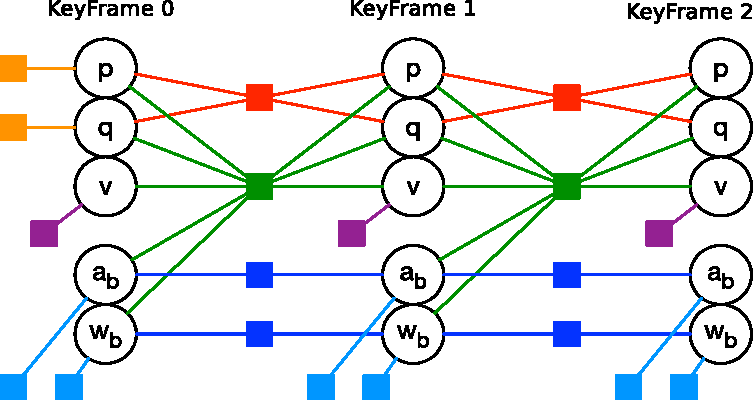
\includegraphics[scale=0.65]{figures/graph_exploded}
%\par\vspace{4mm}
%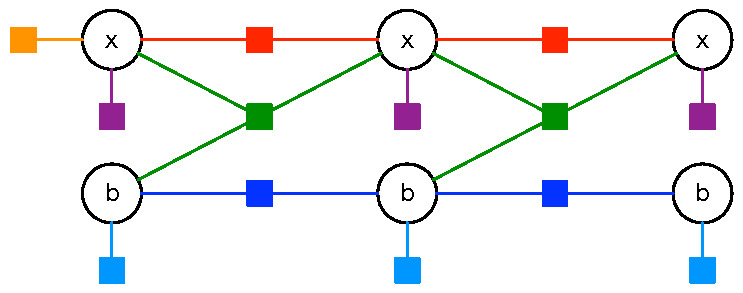
\includegraphics[scale=0.65]{figures/graph_simplified}
\par\vspace{4mm}
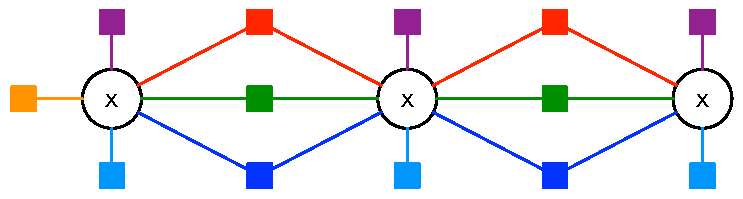
\includegraphics[scale=0.65]{figures/graph_essential}
\caption{
{\bf Top}: Detailed factor graph for the initial keyframe and two steps. \emph{Circles}: state blocks for position ($p$), orientation quaternion ($q$), velocity ($v$), accelerometer bias ($a_b$), gyrometer bias ($\omega_b$). \emph{Orange}: initial pose factor. \emph{Red}: leg kinematic factor. \emph{Green}: IMU's delta pre-integration factor. 
\emph{Blue}: bias drift factor. \emph{Cyan}: bias absolute factor. \emph{Purple}: zero-velocity factor. 
%{\bf Mid}: Simplified factor graph where aggregate state blocks $x=(p,q,v)$ and biases $b=(a_b,\omega_b)$ are used. 
{\bf Bottom}: Equivalent factor graph with one aggregate state block $x=(p,q,v,a_b,\omega_b)$ for each key-frame. All factors are affecting exactly the same variables as in the Top graph.
}
\label{default}
\end{center}
\end{figure}

%\begin{figure}[htbp]
%\begin{center}
%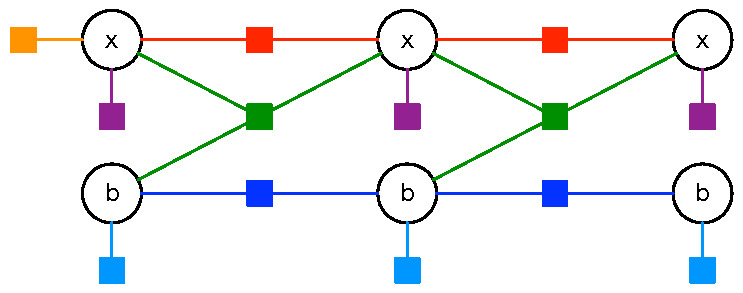
\includegraphics[scale=0.65]{figures/graph_simplified}
%\caption{default}
%\label{default}
%\end{center}
%\end{figure}


% !TEX root = main.tex





\section{IMU pre-integration in S3 and SO(3)}
\label{sec:imu}

%%%%%%%%%%%%%%%%%%%%%%%%%%%%%%%%%%%%%%%%%%%%%%%%%%%%%%%%%%%%
\subsection{Overview}

Due to the different rates of IMU data and keyframe (KF) creations, hundreds of IMU measurements need to be integrated to generate a motion factor linking two consecutive KFs. 
The integration of the motion equations in an absolute reference frame strongly depends on the initial conditions of orientation, velocity and IMU bias.
Therefore, the changes in the estimates of these magnitudes (inherent to the iterative nature of the optimization) affect the whole motion integral. 
Delta pre-integration theory was developed to avoid the need of re-integrating all IMU data at each iteration \cite{LUPTON-09,forster2015imu}. 
On the one hand, this theory defines new motion magnitudes called \emph{deltas}, which are independent of the initial conditions of orientation and velocity, and thus depend \emph{only} on the IMU data and bias. 
On the other hand, the effect of the changes in the bias estimates is linearized so that the deltas can be corrected a posteriori, 
\ie, when computing the residual, 
using pre-computed Jacobians. 

In this section, we revise the IMU pre-integration theory, providing three contributions: 
1) a segmentation of the computation pipeline (from measurements, to body magnitudes, to the current delta, and to the integrated delta); 
2) a physical interpretation of the delta magnitudes; 
and 
3) a simpler yet rigorous algebraic approach, valid for both the S3 (quaternion) and SO3 (rotation matrix) manifolds, which takes profit of the pipeline segmentation and the chain rule to compute the otherwise combersome Jacobians \cite{forster2015imu}. 
Important complements are provided in \appRef{sec:derivatives_SO3} for the sake of background and completeness.

%%%%%%%%%%%%%%%%%%%%%%%%%%%%%%%%%%%%%%%%%%%%%%%%%%%%%%%%%%%%
\subsection{Quaternion rotations}

We define the quaternion-by-vector product $\od$ so that
%
\begin{align}
\bfq\od\bfv \te \bfq\ot\bfv\ot\bfq^*
~,
\end{align}
%
where the symbol $\ot$ indicates the quaternion product.
That is, quaternion-by-vector products using the symbol $\od$ perform 3D rotations. 
Notice that if $\bfR$ is the rotation matrix equivalent to the quaternion $\bfq$, then 
%
$\bfq\od\bfv = \bfR\,\bfv$. 
%
This straightforward equivalence
enables us to define all the forthcoming IMU pre-integration algebra in a way that allows a direct passage between the $S3$ (quaternion) and $SO(3)$ (rotation matrix) implementations.




%%%%%%%%%%%%%%%%%%%%%%%%%%%%%%%%%%%%%%%%%%%%%%%%%%%%%%%%%%%%

\subsection{State integration in the absolute reference frame}

We define the world-referenced states of position, velocity, and orientation quaternion, $\bfx\!=\!(\bfp,\bfv,\bfq)$. 
Their time evolution is governed by the kinematic equation,
%
\begin{align}\label{equ:cont_basic}
\begin{split}
\dot\bfp &= \bfv \\
\dot\bfv &= \bfg + \bfq\od\bfa \\
\dot\bfq &= \frac12\bfq\ot\bw 
\end{split}
\end{align}
%
where we identify $\bfb=(\bfa,\bw)$ as the \emph{body magnitudes}, that is, the magnitudes of acceleration and angular rate observed at the IMU reference frame. These are obtained at discrete times $t_j$ from biased and noisy IMU measurements, \ie,
%
\begin{align}\label{equ:body}
\begin{split}
\bfa_j &\te \bfa_{m,j} - \bfa_{b,j} - \bfa_n \\
\bw_j  &\te \bw_{m,j}  - \bw_{b,j}  - \bw_n 
~,
\end{split}
\end{align}
%
with $\bullet_m$ the measurements, $\bullet_b$ the biases, and $\bullet_n$ the noises.
Assuming constant body magnitudes within the IMU sampling period $\dt\te t_k-t_j$, we have the discrete-time relation
%
\begin{align}\label{equ:integration_state}
\begin{split}
\bfp_{k} &= \bfp_j + \bfv_j\dt  + \frac12\bfg\dt^2 + \frac12\bfq_j\od\bfa_j\dt^2 \\
\bfv_{k} &= \bfv_j + \bfg\dt + \bfq_j\odot\bfa_j\dt \\
\bfq_{k} &= \bfq_j\ot\Exp(\bw_j\dt/2) 
\end{split}
\end{align}


%%%%%%%%%%%%%%%%%%%%%%%%%%%%%%%%%%%%%%%%%%%%%%%%%%%%%%%%%%%%
\subsection{Delta definitions}

Consider a non-rotating reference frame that is free-falling at the acceleration of gravity $\bfg$, and name it $\cG_t$. 
An ideal (unbiased and noiseless) IMU glued to this frame would measure null accelerations and rotations. 
Any non-null measurements would imply motion of the IMU \wrt  $\cG_t$.

At $t=t_i$, we initialize $\cG_i$ at $\bfx_i=(\bfq_i,\bfv_i,\bfq_i)$.
At a later time $t=t_j$,  $\cG_j$ has fallen according to $\bfg$, and the state of our moving body is at $\bfx_j=(\bfq_j,\bfv_j,\bfq_j)$.
The motion delta, denoted $\D_{ij}
$, is defined as the state (position, velocity, orientation) of our body \wrt  $\cG_j$, that is,
%
\begin{align}\label{equ:delta_definition}
\begin{split}
\Dp_{ij} &= \bfq_i^*\od\Big(\bfp_j - \bfp_i - \bfv_i\Dt_{ij} - \frac12\bfg\Dt_{ij}^2\Big) \\
\Dv_{ij} &= \bfq_i^*\od(\bfv_j - \bfv_i - \bfg\Dt_{ij}) \\
\Dq_{ij} &= \bfq_i^*\ot\bfq_j 
\end{split}
\end{align}
%
where $\Dt_{ij} \te t_j - t_i$. 
Notice that this definition is the same provided in \cite{LUPTON-09,forster2015imu}, and that we have given it a clear physical meaning.
Interestingly, the deltas form a group under the composition $\D_{ik}\te\D_{ij}\oplus\D_{jk}$, defined by,
%
\begin{align} \label{equ:composition}
\begin{split}
\Dp_{ik} 
&= \Dp_{ij} + \Dv_{ij}\Dt_{jk} + \Dq_{ij}\od\Dp_{jk} \\
\Dv_{ik} 
&= \Dv_{ij} + \Dq_{ij}\od\Dv_{jk} \\
\Dq_{ik} 
&= \Dq_{ij}\ot\Dq_{jk} 
\end{split}
\end{align}
%
with identity $\D_0=[(0,0,0),(0,0,0),(1,0,0,0)]$, and inverse $\D_{ji}\te\D_{ij}\inv$ shuch that $\D\inv\op\D=\D\oplus\D\inv=\D_0$ (the inverse expression is not given for space reasons).
At any time $j$ we can recover the state estimate $\bfx_j$ given the state estimate $\bfx_i$ and the delta $\D_{ij}$,
%
\begin{align} \label{equ:reconstruction}
\begin{split}
\bfp_j &= \bfp_i + \bfv_i\Dt_{ij} + \frac12\bfg\Dt_{ij}^2 + \bfq_i\od\Dp_{ij} \\
\bfv_j &= \bfv_i + \bfg\Dt_{ij} + \bfq_i\od\Dv_{ij} \\
\bfq_j &= \bfq_i\ot\Dq_{ij}   
\end{split}
\end{align}

%%%%%%%%%%%%%%%%%%%%%%%%%%%%%%%%%%%%%%%%%%%%%%%%%%%%%%%%%%%%
\subsection{Incremental delta pre-integration}

Substituting the integration equation \eqRef{equ:integration_state} in the delta definitions \eqRef{equ:delta_definition}, we obtain the incremental delta pre-integration,
%
\begin{align}\label{equ:g_second_order_pre-integration}
\begin{split}
\Dp_{ik} 
&= \Dp_{ij} + \Dv_{ij}\dt + \frac12\Dq_{ij}\od\bfa_j\dt^2 \\
\Dv_{ik} 
&= \Dv_{ij} + \Dq_{ij}\od\bfa_j\dt \\
\Dq_{ik} 
&= \Dq_{ij}\ot\Exp(\bw_j\dt) 
\end{split}
\end{align}
%
which starts at $\D_{ii}=\D_0$, being $t_i$ the time of the last KF. Interestingly, \eqRef{equ:g_second_order_pre-integration} is analogous to the motion of a body \emph{in an inertial frame} under constant acceleration and rotation rate.
Notice that by letting the reference frame fall with gravity, we get rid of the dependence on gravity of the integration equations, and the only magnitudes entering the integral are the body magnitudes.
Notice also that we can define a proper delta $\delta_{jk}$ from the current body magnitudes $\bfb_j=(\bfa_j,\bw_j) \te \bfb_{m,i} - \bfb_{b,j} - \bfb_{n,j}$ at time $t_j$,
%
\begin{align}\label{equ:delta_creation}
\begin{split}
\dpp_{jk} &= \frac12\bfa_j\dt^2 \\
\dv_{jk} &= \bfa_j\dt \\
\dq_{jk} &= \Exp(\bw_j\dt)
\end{split}
\end{align}
%
%(notice that $\bfb_{b,j}=\bfb_{b,i}$) 
and write the integration \eqRef{equ:g_second_order_pre-integration} as the composition 
%
\begin{align}\label{equ:composition_compact}
\D_{ik}=\D_{ij}\oplus\delta_{jk}
\end{align}
%
described in \eqRef{equ:composition}. 
Typically, we take the biases at KF time $t_i$, that is, $\bfb_{b,j} = \bfb_{b,i}$.
In the following, we will identify $\D$ with the pre-integrated delta, and $\delta$ with the current delta.


%%%%%%%%%%%%%%%%%%%%%%%%%%%%%%%%%%%%%%%%%%%%%%%%%%%%%%%%%%%%
\subsection{Jacobians}

\newcommand{\jac}[2]{{\bfJ^{#1}_{#2}}}

%Notation: 
We note all Jacobians with $\jac{y}{x}\te\dparil{y}{x}$ and refer the reader to \appRef{sec:derivatives_SO3} for details on the development of all non-trivial Jacobian blocks in this section.



\subsubsection{Jacobians of the body magnitudes}

We have from \eqRef{equ:body},
%
\begin{align}\label{equ:jac_body}
\jac{\bfb}{\bfb_m}&=\bfI_6 & \jac{\bfb}{\bfb_b}&=-\bfI_6 & \jac{\bfb}{\bfb_n}&=-\bfI_6
~.
\end{align}

\subsubsection{Jacobians of the current delta}
\label{sec:jac_data}

We have from \eqRef{equ:delta_creation},
%
\begin{align}\label{equ:jac_current_delta}
\jac{\delta_{jk}}{\bfb_j} =
\begin{bmatrix}
\frac12\bfI\dt^2 	& \bf0 \\
\bfI\dt 			& \bf0 \\
\bf0 	          & \bfJ_r(\bw_j\dt)\dt
\end{bmatrix} 
\in \bbR^{9\tcross6}
\end{align}
%
where we develop the lower-right block as in \appRef{sec:jac_R3toSO3}.





\subsubsection{Jacobians of the delta composition}

We differentiate the delta composition \eqRef{equ:composition_compact} described in \eqRef{equ:composition},
%
\begin{subequations}\label{equ:jac_composition}
\begin{align}
\jac{\D_{ik}}{\D_{ij}} &= \begin{bmatrix}
\bfI  & \bfI\dt & - \DR_{ij}  \hatx{\dpp_{jk}}  \\
\bf0  & \bfI    & - \DR_{ij}  \hatx{\dv_{jk}} \\
\bf0  & \bf0    &   \dR_{jk}\tr 
\end{bmatrix} 
\in \bbR^{9\tcross9}
\\
\jac{\D_{ik}}{\delta_{jk}} &= \begin{bmatrix}
\DR_{ij} & \bf0     & \bf0 \\
\bf0     & \DR_{ij} & \bf0 \\
\bf0     & \bf0     & \bfI  
\end{bmatrix}
~~~~~~~~~\in \bbR^{9\tcross9}
\end{align}
\end{subequations}
%
where $\DR_{ij}$ and $\dR_{jk}$ are the rotation matrix deltas corresponding to the respective quaternion deltas $\Dq_{ij}$ and $\dq_{jk}$. 
We develop all the non-trivial blocks as in \appRef{sec:jac_SO3xR3toR3}.


%%%%%%%%%%%%%%%%%%%%%%%%%%%%%%%%%%%%%%%%%%%%%%%%%%%%%%%%%%%%
\subsection{Incremental delta covariance integration}

Let $\bfQ_\D$ be the covariance of the pre-integrated delta, and $\bfQ_n$ that of the measurement noise. For convenience, we first compute the covariance of the current delta,
%
\begin{align}
\bfQ_\delta =  \jac{\delta}{\bfb_n}\bfQ_n\,\jac{\delta}{\bfb_n}\tr
~,
\end{align}
%
where $\jac{\delta}{\bfb_n} = \jac{\delta}{\bfb} \cdot \jac{\bfb}{\bfb_n}
$ is the noise Jacobian, obtained with \eqsRef{equ:jac_body}{equ:jac_current_delta} and the chain rule.
The delta covariance is then integrated with
%
\begin{align}
\bfQ_{\D_{ik}} = \jac{\D_{ik}}{\D_{ij}}\bfQ_{\D_{ij}}\,\jac{\D_{ik}}{\D_{ij}}\tr + \jac{\D_{ik}}{\delta_{jk}}\bfQ_\delta\,\jac{\D_{ik}}{\delta_{jk}}\tr
~,
\end{align}
%
using Jacobians \eqRef{equ:jac_composition}, and starting at $\bfQ_{\D_{ii}}={\bf0}_{9\tcross9}$.



%%%%%%%%%%%%%%%%%%%%%%%%%%%%%%%%%%%%%%%%%%%%%%%%%%%%%%%%%%%%
\subsection{Delta correction with new bias}

Let $\ol\D$ and $\ol{\bfb_b}$ be respectively the pre-integrated delta and the bias values used during pre-integration. Since the bias estimates change at each iteration of the optimizer, we need to update the delta according to the new bias values $\bfb_b$. We do so with the linearized update,
%
\begin{align}\label{equ:delta_correction}
\D = \ol\D + \jac{\D}{\bfb_b}(\bfb_b - \ol{\bfb_b})
~,
\end{align}
%
where $\jac{\D}{\bfb_b}$ is the pre-integrated bias Jacobian, computed incrementally using also the chain rule,
%
\begin{align}
\jac{\D_{ik}}{\bfb_b} 
= \jac{\D_{ik}}{\D_{ij}}\jac{\D_{ij}}{\bfb_b} 
- \jac{\D_{ik}}{\delta_{jk}}\jac{\delta_{jk}}{\bfb_b}
~.
\end{align}
%
with 
$
\jac{\delta_{jk}}{\bfb_b}=\jac{\delta_{jk}}{\bfb} \jac{\bfb}{\bfb_b}
$.
%
This Jacobian starts at $\jac{\D_{ii}}{\bfb_b} = {\bf0}_{9\tcross 9}$.


%%%%%%%%%%%%%%%%%%%%%%%%%%%%%%%%%%%%%%%%%%%%%%%%%%%%%%%%%%%%
\subsection{Residual}

The computation of the residuals for the IMU delta factors (see \figRef{fig:factor_graph}, green) requires: the state estimates $\bfx_i$ and $\bfx_j$; the current bias estimates $\bfb_{b,i}$; the pre-integrated delta $\ol{\D_{ij}}$; the bias used during pre-integration $\ol{\bfb_{b,i}}$; and the pre-integrated bias Jacobian $\jac{\D_{ij}}{\bfb_b}$. The process is best understood if split into smaller steps: we first compute a corrected delta $\D_{ij}$ using \eqRef{equ:delta_correction}; then compute a predicted delta $\widehat\D_{ij}$ using \eqRef{equ:delta_definition}; and finally compute the residual with
%
\begin{align}\label{equ:imu_residual}
\bfr(\bfx_i,\bfx_j,\bfb_{b,i}) 
= \begin{bmatrix}
\Dp_{ij}-\widehat\Dp_{ij} \\
\Dv_{ij}-\widehat\Dv_{ij} \\
\Log(\widehat\Dq_{ij}^*\ot\Dq_{ij})
\end{bmatrix} 
\in \bbR^9
~.
\end{align}
%
Its information matrix is given by $\bfOmega=\bfQ_{\D ik}\inv$.







% !TEX root = main.tex

\section{Experiments} \label{sec:experiments}

The confidence one can have on the encoders of the robot depends on several factors from actuators design to control strategies. in the legged locomotion case, this can also depend on the general design of the robot.
Thus during walking phases with humanoid robot HRP2, one can notice sliding phenomenon when the foot hits the ground. If this effect is not measured, their occurrences can turn to be a problem for navigation in unstructured environment. 
Furthermore, we cannot anticipate the sliding, meaning that we do not know what actually causes this to happen. 
In this context, we show that measuring this slide and getting a better estimation of both real trajectories and real position of the foot is possible with an IMU fixed on the sliding member, the foot of the robot in our case.

In order to get to that point, we first want to check whether our fusion method of both IMUs and odometer is able to get a correct estimation of one's foot during walking.
Then we show that using an IMU on the foot of the robot leads to a better estimation of the real position of the member compared to encoder based odometry.

We chose to use a low-cost IMU in our application to realize the feasibility of our method. For this purpose we selected the 
MPU6050 from Invensense combining both an accelerometer and a gyroscope and extensively used in the open source community.


%\textit{Keywords : low-cost IMU, MPU6050, experiment conditions, 1 KHz IMU} \\
%\textit{TODO : add factor graph for experiment visualization}

\subsection{Method}
\subsubsection{auto-calibration}

The parameters we need to calibrate for a correct integration are the biases on top of which we integrate the incoming data of the IMU.
The time varying property of the bias is a critical point to consider in order to avoid large deviations. This calibration is made possible
by dependencies of the delta pre-integration ($\boldsymbol{\Delta P}(ab, \omega b), \boldsymbol{\Delta V}(ab, \omega b), \boldsymbol{\Delta Q}(\omega b)$). Fusing both odometer and IMU provides constraints on position and orientation parts of
the state vector. However, velocity is still not observable and is affected by the bias estimation. In the case of legged locomotion, we fix the observability problem by adding a zero velocity constraint when the foot is on the ground.

The initial orientation estimation is made possible by adding an absolute constraint on yaw part of the state vector, otherwise we would run in observability problems. \textbf{add figure here (graph)}

\subsection{Results}
\subsubsection{Trajectory reconstruction}

We check the feasibility of the trajectory reconstruction using a 1Khz IMU attached to one's foot tracked with a motion capture (MOCAP) system. The MOCAP is used to get odometry between zero-velocity phases, i.e. when the foot is on the ground,
and will be taken as the ground truth against which we compare the trajectory reconstruction.

We reproduce the movements the feet of a robot could have when it is walking. However, as shown in figures \textbf{add figure here}, the final optimal state
is not the expected one and acceleration biases are rapidly changing. The variation that we can see is not only due to some random walk and can be explained by the excitement of biases in a different axis.
As explained in \cite{roussillon2011rt}, in opposition to gyroscope biases, acceleration biases do not converge toward stable values during a motion exciting several axis of the sensor. 
This effect can be explained by time inconsistency meaning that we fail
to use the information of the entire motion to converge toward stable values as expected in the sensor model, but the problem may also be that the step motions do not use all the axis of the accelerometer as it should.

We fix the trajectory estimation problem by adding odometry information during foot's flying phase. However, we cannot fix any other conditions making velocity and bias observation possible hence all parameters of the state vector are estimated.
This added KeyFrame reduces the integration time since last state optimization making bias random walk variation less critical on estimation. As we can see, results are much better and closer to MOCAP's ground truth as we could expect.

%TODO : process mocap experiments

\subsubsection{Legged-Locomotion's undesired behavior measurement}

We use the approach presented above in the case of the humanoid robot HRP2 to better estimate the trajectory of the foot. This also results in a better estimation of the pose of the robot using its kinematic chain. 
For this experiment, the robot is moving in open loop and some particularities are worth to be noted compared to previous experiment. 
The structure of the robot produces vibrations that are measured by the IMU, thus explaining the over noisy aspect of the data. The foot's flying phase is set to last 800 ms. The double support phase lasts only 20 ms, thus it is difficult to observe
even with the IMU working at 1 KHz because of the vibration it will measure on impacts.




%TODO experiment : step motion + complex rotation, followed by MOCAP



% !TEX root = main.tex

\section{Conclusion}

We have presented a method to measure foot movement during robot biped locomotion. We fuse information from an IMU attached to the foot, the kinematic chain measured by the robot encoders, and available knowledge extracted from the gait phases, such as zero velocity and IMU bias dynamics. We used nonlinear optimization techniques based on factor graphs, which has proved to be a flexible and powerful fusion framework. For this, we have revised the IMU pre-integration theory, and proposed an implementation in the quaternions manifold, with simpler derivations than previous works, and with physical interpretations, which we believe go in the direction of improving the clarity of the method.


Results showed that this estimation method is able to detect subtle movements that are not measurable using the encoders alone, such as a sliding foot condition at the beginning or end of the contact phase. These slides, if undetected, have a dramatic negative impact on the overall robot odometry.

% !TEX root = main.tex

%%%%%%%%%%%%%%%%%%%%%%%%%%%%%%%%%%%%%%%%%%%%%%%%%%%%%%%%%%%%
\appendix

\section{Definition of the derivatives }

\subsection{The additive and subtractive operators in $SO(3)$}

In vector spaces $\bbR^n$, the addition and subtraction operations are performed with the regular sum `$+$' and minus `$-$' operations.
In $SO(3)$ this is not possible, but equivalent operators are needed for establishing a proper calculus corpus. 

We thus define the plus and minus operators, $\oplus,\ominus$, between elements $\sR\in SO(3)$, and elements $\bth\in\bbR^3$ of the tangent space at $\sR$, as follows.

\paragraph{The plus operator.}
The `plus' operator $\oplus:SO(3)\times\bbR^3\to SO(3)$ produces an element $\sS$ of $SO(3)$ which is the result of composing a reference element $\sR$ of $SO(3)$ with a (often small) rotation specified by a vector of $\bth\in\bbR^3$ in the vector space tangent to the reference element $\sR$,
%
\begin{align}
\sS = \sR\oplus \bth &\te \sR\circ\Exp(\bth) && \sR,\sS\in SO(3),~ \bth\in\bbR^3 
\end{align}
%
Notice that this operator may be defined for any representation of $SO(3)$. In particular, for the quaternion and rotation matrix we have,
%
\begin{align}
\bfq_\sS &= \,\bfq_\sR\oplus\bth = \bfq_\sR\ot\Exp(\bth) \\
\bfR_\cS &= \bfR_\sR\oplus \bth = \bfR_\sR\Exp(\bth) 
\end{align}

\paragraph{The minus operator.}
The `minus' operator $\ominus:SO(3)\times SO(3)\to\bbR^3$ is the inverse of the above. It returns the vectorial angular difference $\bth\in\bbR^3$ between two elements of $SO(3)$. This difference is expressed in the  vector space tangent to the reference element $\sR$, 
%
\begin{align}
\bth=\sS\ominus \sR
&\te \Log(\sR\inv \circ \sS)     && \sR,\sS\in SO(3),~ \bth\in\bbR^3  
\end{align}
%
which for the quaternion and rotation matrix reads,
%
\begin{align}
\bth &= \,\,\bfq_\sS\ominus\bfq_\sR\, = \Log(\bfq_\sR^*\ot\bfq_\sS)                      \\
\bth &= \bfR_\sS\ominus\bfR_\sR = \Log(\bfR_\sR\tr\,\bfR_\sS)                         
\end{align}

\bigskip
In both cases, notice that even though the vector difference $\bftheta$ is typically supposed to be small, the definitions above hold for any value of $\bftheta$ (up to the first coverage of the $SO(3)$ manifold, that is, for angles $\theta<\pi$).

\subsection{The four possible derivative definitions}



\subsubsection{Functions from vector space to vector space}

The scalar and vector cases follow the classical definition of the derivative: given a function $f:\bbR^m\to\bbR^n$, we use $\{+,-\}$ to define the derivative as
%
\begin{align}
\dpar{f(\bfx)}{\bfx} &\te \lim_{\delta\bfx\to0}\frac{f(\bfx+\delta\bfx)-f(\bfx)}{\delta\bfx} &&\in \bbR^{n\times m} \label{equ:derivative_vector}
\end{align}
%
Euler integration produces linear expressions of the form
%
\begin{align*}
f(\bfx+\Delta\bfx) &\approx f(\bfx) + \dpar{f(\bfx)}{\bfx}\Delta\bfx
& \in \bbR^n
\end{align*}

\subsubsection{Functions from $SO(3)$ to $SO(3)$}

Given a function $f:SO(3) \to SO(3)$ with $\sR\in SO(3)$ and a local, small angular variation $\bth\in\bbR^3$, we use $\{\oplus,\ominus\}$ to define the derivative as
%
\begin{align}
\dpar{f(\sR)}{\bth} 
&\te \lim_{\delta\bth\to0}\frac{f(\sR\oplus\delta\bth)\ominus f(\sR)}{\delta\bth}  && \in \bbR^{3\times 3}\\
&= \lim_{\delta\bth\to0}\frac{\Log\big(f\inv(\sR)\,f(\sR\Exp(\delta\bth))\big)}{\delta\bth} \label{equ:derivative_SO3}
\end{align}
%
Euler integration produces expressions of the form,
%
\begin{align*}
f(\sR\oplus\Delta\bth) &\approx f(\sR)\,\oplus\,\dpar{f(\sR)}{\bth}\,\Delta\bth
 \te f(\sR)\Exp\left(\dpar{f(\sR)}{\bth}\Delta\bth\right)
 & \in SO(3)
\end{align*}




\subsubsection{Functions from vector space to $SO(3)$}

For the case of a function $f:\bbR^m\to SO(3)$, we use `+' for the vector perturbations, and `$\ominus$' for the $SO(3)$ difference,
%
\begin{align}
\dpar{f(\bfx)}{\bfx} &\te \lim_{\delta\bfx\to0} \frac{ f(\bfx+\delta\bfx)\ominus f(\bfx)}{\delta\bfx} && \in \bbR^{3\times m} \label{equ:dif_RtoSO3}\\
&= \lim_{\delta\bfx\to0} \frac{\Log(f\inv(\bfx) f(\bfx+\delta\bfx))}{\delta\bfx}
\end{align}
%
Euler integration produces expressions of the form,
%
\begin{align*}
f(\bfx+\Delta\bfx) &\approx f(\bfx)\,\oplus\,\dpar{f(\bfx)}{\bfx}\,\Delta\bfx
 \te f(\bfx)\,\Exp\left(\dpar{f(\bfx)}{\bfx}\Delta\bfx\right)
 & \in SO(3)
\end{align*}

\subsubsection{Functions from $SO(3)$ to vector space}

For the case of a function $f: SO(3)\to\bbR^n$, we use `$\oplus$' for the $SO(3)$ perturbations, and `$-$' for the vector difference,
%
\begin{align}
\dpar{f(\sR)}{\bth} &\te \lim_{\delta\bth\to0} \frac{f(\sR\oplus\delta\bth) - f(\sR)}{\delta\bth} && \in \bbR^{n\times 3} \label{equ:jacobian_SO3_Rn}\\
&= \lim_{\delta\bth\to0} \frac{f(\sR\Exp(\delta\bth)) - f(\sR)}{\delta\bth}
\end{align}
%
Euler integration produces expressions of the form,
%
\begin{align*}
f(\sR\oplus\delta\bth) &\approx f(\sR)+\dpar{f(\sR)}{\bth}\,\Delta\bth
 \te f(\sR)+\Exp\left(\dpar{f(\sR)}{\bth}\Delta\bth\right)
 & \in SO(3)
\end{align*}


\subsection{Right Jacobian of $SO(3)$ }

We define the right Jacobian of $SO(3)$ as, 
%
\begin{align}
\bfJ_r(\bth) &\te \dpar{\Exp(\bth)}{\bth} 
\end{align}
%
Since the exponential $\Exp()$ is an application $\bbR^3\to SO(3)$,
we implement this derivative using \eqRef{equ:dif_RtoSO3},
%
\begin{align}
\bfJ_r(\bth) &= \lim_{\dth\to0}\frac{\Exp(\bth+\dth)\ominus\Exp(\bth)}{\dth} \\
 &= \lim_{\dth\to0}\frac{\Log(\Exp(\bth)\tr\Exp(\bth+\dth))}{\dth} && \textrm{if using $\bfR$} \\
 &= \lim_{\dth\to0}\frac{\Log(\Exp(\bth)^*\ot\Exp(\bth+\dth))}{\dth} && \textrm{if using $\bfq$} 
 ~.
\end{align}
%
It has the properties, for any $\bth$ and small $\dth$,
%
\begin{align}
\Exp(\bth+\dth) &\approx \Exp(\bth)\Exp(\bfJ_r(\bth)\dth) \\
\Exp(\bth)\Exp(\dth) &\approx \Exp(\bth+\bfJ_r\inv(\bth)\,\dth) \\
\Log(\Exp(\bth)\Exp(\dth)) &\approx \bth+\bfJ_r\inv(\bth)\,\dth 
\end{align}

The right Jacobian and its inverse can be computed in closed form with
%
\begin{align}
\bfJ_r(\bth) &= \bfI - \frac{1-\cos\nth}{\nth^2}\hatx{\bth} + \frac{\nth-\sin\nth}{\nth^3}\hatx{\bth}^2 \\
\bfJ_r\inv(\bth) &= \bfI + \frac12\hatx{\bth} + \left(\frac1{\nth^2} - \frac{1+\cos\nth}{2\nth\sin\nth}\right)\hatx{\bth}^2
\end{align}






%%%%%%%%%%%%%%%%%%%%%%%%%%%%%%%%%%%%%%%%%%%%%%%%%%%%%%%%%%%%%%%%%%%%%%%%%%%
\section{Rules, do's and don'ts for Jacobians}
\label{sec:DosDonts}

We provide a collection of rules which come very handy to develop Jacobians. They come organized under helper \com{keys}\!\!\!\!, which we use to refer to each of these properties in our developments.

\subsection{Useful properties: Do's}

\paragraph{\cchain : Chain rule}

\begin{align}
\dpar{\bfz}{\bfx} = \dpar{\bfz}{\bfy}\cdot\dpar{\bfy}{\bfx}
\end{align}

\paragraph{\ccross : Cross product and skew-symmetric matrix}

\begin{align}
\hatx{\bfa}\bfb &= \bfa\times\bfb \\
\hatx{\bfa}\bfb &= -\hatx{\bfb}\bfa \\
\bfR\tr\hatx{\bfR\bfa}\bfR &= \hatx{\bfa} \\
\hatx{\bfR\bfa} &= \bfR\hatx{\bfa}\bfR\tr 
\end{align}

\paragraph{\cJr : Right Jacobian of $SO(3)$ }

It has the properties, for any $\bth$ and small $\dth$,
%
\begin{align}
\Exp(\bth+\dth) &\approx \Exp(\bth)\Exp(\bfJ_r(\bth)\dth) \\
\Exp(\bth)\Exp(\dth) &\approx \Exp(\bth+\bfJ_r\inv(\bth)\,\dth) \\
\Log(\Exp(\bth)\Exp(\dth)) &\approx \bth+\bfJ_r\inv(\bth)\dth %\\
\end{align}
%






\paragraph{\csmall : Small angle approximations}

Let $\dth$ be a small angle vector. Then,
%
\begin{align}
\Exp(\dth) &\approx \bfI + \hatx{\dth} \\
\Exp(\dth)\tr &\approx \bfI - \hatx{\dth} \\
\Exp(\dth_1)\Exp(\dth_2) &\approx \Exp(\dth_1+\dth_2) \\
\textstyle\prod_i \Exp(\dth_i) &\approx \Exp\!\big(\textstyle\sum_i\dth_i\big) \\
\bfJ_r(\dth) &\approx \bfI - \frac12\hatx{\dth} \\
\bfJ_r\inv(\dth) &\approx \bfI + \frac12\hatx{\dth} 
\end{align}
%
Example: we often use $\Exp(\bfJ_r(\bth)\dth)\approx \bfI + \hatx{\bfJ_r(\bth)\dth}$.

\paragraph{\cswap : Reversing product order}

Since $$\bfR\Exp(\bth)\bfR\tr=\bfR\exp(\hatx{\bth})\bfR\tr=\exp(\bfR\hatx{\bth}\bfR\tr)=\exp(\hatx{\bfR\bth})=\Exp(\bfR\bth),$$ then
%
\begin{align}
\Exp(\bth)\bfR &= \bfR\Exp(\bfR\tr\bth) \\
\bfR\tr\Exp(\bth)\bfR &= \Exp(\bfR\tr\bth) \\
\Exp(\bth)\Exp(\bphi) &= \Exp(\bphi)\Exp(\Exp(\bphi)\tr\bth) 
\end{align}


\paragraph{\cexpand, \csubst, \ccancel : Expand, substitute, cancel :} This happens when we expand or substitute a previously defined term, or when we cancel terms.

\paragraph{\tcom{$\oplus$}, \tcom{$\ominus$}, \tcom{(1)} : Apply definition :} This happens when we apply a particular definition or equation number.

\subsection{Common mistakes: Don'ts}

\begin{align}
\Exp(\bth_1+\bth_2) &\ne \Exp(\bth_1)\Exp(\bth_2) \\
\Log(\bfR_1\bfR_2) &\ne \Log(\bfR_1) + \Log(\bfR_2) \\
\bfJ_r(\bth) &\ne \bfI - \frac12\hatx{\bth} \\
\bfJ_r\inv(\bth) &\ne \bfI + \frac12\hatx{\bth} 
\end{align}
%
however, these hold approximately true for small angle vectors. See \csmall above.


\subsection{Examples}

\subsubsection{Example 1: $\bbR^3\times\bbR^3\to\bbR^3$} 

The rotation $f(\bth,\bfv) = \bfR(\bth)\,\bfv = \Exp(\bth)\,\bfv \in \bbR^3$ produces vectors of $\bbR^3$ from vectors $\bth,\bfv$ in $\bbR^3$. Its Jacobians are defined by \eqRef{equ:derivative_vector} and developed as
%
\begin{align*}
\dpar{\bfR(\bth)\bfv}{\bth} 
&= \lim_{\delta\bth\to0}\frac{\Exp(\bth+\delta\bth)\bfv-\Exp(\bth)\bfv}{\delta\bth} \\
\cJr
&= \lim_{\delta\bth\to0}\frac{\Exp(\bth)\Exp(\bfJ_r(\bth)\delta\bth)\bfv-\Exp(\bth)\bfv}{\delta\bth} \\
\csmall
&= \lim_{\delta\bth\to0}\frac{\Exp(\bth)(\bfI+\hatx{\bfJ_r(\bth)\delta\bth})\bfv-\Exp(\bth)\bfv}{\delta\bth} \\
\ccancel
&= \lim_{\delta\bth\to0}\frac{\Exp(\bth)\hatx{\bfJ_r(\bth)\delta\bth}\bfv}{\delta\bth} \\
\ccross
&= \lim_{\delta\bth\to0}\frac{-\Exp(\bth)\hatx{\bfv}\bfJ_r(\bth)\delta\bth}{\delta\bth} \\
&= -\bfR(\bth)\hatx{\bfv}\bfJ_r(\bth) 
\end{align*}
%
and
%
\begin{align*}
\dpar{\bfR(\bth)\bfv}{\bfv} 
&= \lim_{\partial\bfv\to0}\frac{\bfR(\bth)(\bfv+\partial\bfv)-\bfR(\bth)\bfv}{\partial\bfv} \\
\com{cancel} 
&= \bfR(\bth)
\end{align*}

\subsubsection{Example 2: $SO(3)\times\bbR^3\to\bbR^3$} 

The rotation $f(\bfR,\bfv) = \bfR\,\bfv \in \bbR^3$ produces vectors of $\bbR^3$ from elements $\bfR\in SO(3)$ and vectors in $\bbR^3$. The first Jacobian is defined by \eqRef{equ:jacobian_SO3_Rn} and developed as
%
\begin{align*}
\dpar{\bfR\bfv}{\bth} 
&\te \lim_{\delta\bth\to0}\frac{(\bfR\oplus\delta\bth)\bfv-\bfR\bfv}{\delta\bth} \\
\com{$\oplus$}
&= \lim_{\delta\bth\to0}\frac{\bfR\Exp(\delta\bth)\bfv-\bfR\bfv}{\delta\bth} \\
\csmall
&= \lim_{\delta\bth\to0}\frac{\bfR\tdot(\bfI+\hatx{\delta\bth})\bfv-\bfR\bfv}{\delta\bth} \\
\ccancel
&= \lim_{\delta\bth\to0}\frac{\bfR\hatx{\delta\bth}\bfv}{\delta\bth} \\
\ccross
&= \lim_{\delta\bth\to0}\frac{-\bfR\hatx{\bfv}\delta\bth}{\delta\bth} \\
&= -\bfR\hatx{\bfv} 
\end{align*}
%
The second Jacobian is defined by \eqRef{equ:derivative_vector} and trivially develops as,
%
\begin{align*}
\dpar{\bfR\bfv}{\bfv} 
&\te \lim_{\partial\bfv\to0}\frac{\bfR\tdot(\bfv+\partial\bfv)-\bfR\bfv}{\partial\bfv} \\
&= \bfR
\end{align*}

\subsubsection{Example 3: $SO(3)\times\bbR^3\to SO(3)$} 

The function $f(\bfR,\bw) = \bfR\Exp(\bw\dt)\in SO(3)$ produces elements of $SO(3)$ from elements in $SO(3)$ and vectors $\bw$ in $\bbR^3$. Its Jacobians are 
%
\begin{align*}
\dpar{\bfR\Exp(\bw\dt)}{\bth} 
&= \lim_{\delta\bth\to0}\frac{(\bfR\oplus\delta\bth)\Exp(\bw\dt)\ominus(\bfR\Exp(\bw\dt))}{\delta\bth} \\
\com{$\oplus,\ominus$}
&= \lim_{\delta\bth\to0}\frac{\Log\big((\bfR\Exp(\bw\dt))\inv \bfR\Exp(\delta\bth)\Exp(\bw\dt)\big)}{\delta\bth} \\
&= \lim_{\delta\bth\to0}\frac{\Log\big(\Exp(\bw\dt)\tr\bfR\tr \bfR\Exp(\delta\bth)\Exp(\bw\dt)\big)}{\delta\bth} \\
\ccancel
&= \lim_{\delta\bth\to0}\frac{\Log\big(\Exp(\bw\dt)\tr\Exp(\delta\bth)\Exp(\bw\dt)\big)}{\delta\bth} \\
\cswap
&= \lim_{\delta\bth\to0}\frac{\Log\big(\Exp(\Exp(\bw\dt)\tr\delta\bth)\big)}{\delta\bth} \\
\ccancel
&= \lim_{\delta\bth\to0}\frac{\Exp(\bw\dt)\tr\delta\bth}{\delta\bth} \\
&= \Exp(-\bw\dt) 
\end{align*}
%
and
%
\begin{align*}
\dpar{\bfR\Exp(\bw\dt)}{\bw} 
&= \lim_{\delta\bw\to0}\frac{\bfR\Exp((\bw+\delta\bw)\dt) \ominus (\bfR\Exp(\bw\dt)) }{\delta\bw} \\
\com{$\ominus$}
&= \lim_{\delta\bw\to0}\frac{\Log\big((\bfR\Exp(\bw\dt))\inv \, \bfR\Exp(\bw\dt+\delta\bw\dt)\big)}{\delta\bw} \\
\cJr
&= \lim_{\delta\bw\to0}\frac{\Log\big((\bfR\Exp(\bw\dt))\inv \bfR\Exp(\bw\dt)\Exp(\bfJ_r(\bw\dt)\delta\bw\dt)\big)}{\delta\bw} \\
\ccancel
&= \lim_{\delta\bw\to0}\frac{\Log\big(\Exp(\bfJ_r(\bw\dt)\delta\bw\dt)\big)}{\delta\bw} \\
\com{cancel}
&= \bfJ_r(\bw\dt)\dt
\end{align*}
%
%This can be seen in a easier way using the chain rule on $\bw\dt$,
%%
%\begin{align*}
%\dpar{\bfR\Exp(\bw\dt)}{\bw} 
%&= \dpar{\bfR\Exp(\bw\dt)}{\bw\dt}\dpar{\bf\dt}{\bw} \\
%&= \dpar{\bfR\Exp(\bw\dt)}{\bw\dt}\dt \\
%\cJr
%&= \bfJ_r(\bw\dt)\dt
%\end{align*}
%
Refer to the text for other developments, \eg~\secRef{sec:jac_first_delta}.



\subsubsection{Example 4: $SO(3)\times SO(3)\to SO(3)$}

The function $f(\bfR,\bfS) = \bfR\{\bftheta\}\,\bfS\{\bfphi\} \in SO(3)$ produces the concatenation of rotations, or rotation composition. Its Jacobians are
%
\begin{align*}
\dpar{\bfR\{\bftheta\}\,\bfS\{\bfphi\}}{\bftheta} 
&= \lim_{\delta\bftheta\to0}\frac{\Log\big((\bfR\bfS)\inv((\bfR\oplus\delta\bftheta)\bfS)\big)}{\delta\bftheta} \\
&= \lim_{\delta\bftheta\to0}\frac{\Log\big((\bfR\bfS)\tr(\bfR\Exp(\delta\bftheta)\bfS)\big)}{\delta\bftheta} \\
&= \lim_{\delta\bftheta\to0}\frac{\Log\big(\bfS\tr\bfR\tr\bfR\Exp(\delta\bftheta)\bfS\big)}{\delta\bftheta} \\
&= \lim_{\delta\bftheta\to0}\frac{\Log\big(\bfS\tr\Exp(\delta\bftheta)\bfS\big)}{\delta\bftheta} \\
\cswap
&= \lim_{\delta\bftheta\to0}\frac{\Log\big(\Exp(\bfS\tr\delta\bftheta)\big)}{\delta\bftheta} \\
&= \lim_{\delta\bftheta\to0}\frac{\bfS\tr\delta\bftheta}{\delta\bftheta} \\
&= \bfS\tr
\end{align*}
%
and
%
\begin{align*}
\dpar{\bfR\{\bftheta\}\,\bfS\{\bfphi\}}{\bfphi} 
&= \lim_{\delta\bfphi\to0}\frac{\Log\big((\bfR\bfS)\tr(\bfR(\bfS\oplus\delta\bfphi))\big)}{\delta\bfphi} \\
&= \lim_{\delta\bfphi\to0}\frac{\Log\big((\bfR\bfS)\tr(\bfR\bfS\Exp(\delta\bfphi))\big)}{\delta\bfphi} \\
&= \lim_{\delta\bfphi\to0}\frac{\Log\big(\Exp(\delta\bfphi)\big)}{\delta\bfphi} \\
&= \lim_{\delta\bfphi\to0}\frac{\delta\bfphi}{\delta\bfphi} \\
&= \bfI
\end{align*}





\section{Uncertainties in $SO(3)$}

\subsection{Description of uncertainty}
\subsubsection{Vector spaces}
\begin{align*}
\widetilde\bfx&=\bfx+\delta\bfx
\end{align*}
\subsubsection{$SO(3)$}
\begin{align*}
\widetilde\bfR&=\bfR\oplus\dth\te\bfR\Exp(\delta\bth) \\
\widetilde\bfq&=\bfq\oplus\dth\te\bfq\ot\Exp(\delta\bth)
\end{align*}

\subsection{Uncertainty propagation}

%
The uncertainty of the composition of two uncertain elements of $SO(3)$ can be derived as follows (we use the matrix form for convenience),
%
\begin{align*}
\widetilde\bfR = \bfR\Exp(\dth) 
&= \widetilde{\bfR_1\bfR_2} \\
&= \widetilde\bfR_1\widetilde\bfR_2 \\
\cexpand
&= \bfR_1\Exp(\dth_1)\bfR_2\Exp(\dth_2) \\
\cswap
&= \bfR_1\bfR_2\Exp(\bfR_2\tr\dth_1)\Exp(\dth_2) \\
\cJr
&\approx \bfR_1\bfR_2\Exp(\bfR_2\tr\dth_1+\bfJ_r\inv(\bfR_2\tr\dth_1)\dth_2) \\
&= \bfR\Exp(\bfR_2\tr\dth_1+\bfJ_r\inv(\bfR_2\tr\dth_1)\dth_2) 
\end{align*}
%
and therefore,
%
\begin{align}
\dth = \bfR_2\tr\dth_1+\bfJ_r\inv(\bfR_2\tr\dth_1)\dth_2
\end{align}
%
We can derive equivalent Jacobian matrices for the propagation. Since each partial derivative assumes null perturbations in  other variables, we have,
%
\begin{align}
\DTH_{\dth_1} \te \dpar{\bth}{\bth_1} &= \frac{\dth(\dth_2=0)}{\dth_1} = \bfR_2\tr \\
\DTH_{\dth_2} \te \dpar{\bth}{\bth_2} &= \frac{\dth(\dth_1=0)}{\dth_2} = \bfI
\end{align}
%
yielding
%
\begin{align}
\dth \approx \bfR_2\tr\dth_1+\dth_2
\end{align}
%
which constitutes a regular frame transformation operation. The covariances are propagated from $\bfR_1$ and $\bfR_2$ to $\bfR$ as 
%
\begin{align*}
\Sigma = \bfR_2\tr\,\Sigma_1\,\bfR_2 + \Sigma_2
\end{align*}


%%%%%%%%%%%%%%%%%%%%%%%%%%%%%%%%%%%%%%%%%%%%%%%%%%%%%%%%%%%%%%%%%%%%%%%%%%%%%%%%
\section*{ACKNOWLEDGMENT}
This work has been supported by EUROC FP7-2013-NMP-ICT-FOF, 
Loco3d ANR-16-CE33-0003, 
the Spanish Ministry of Economy and Competitiveness under Project EB-SLAM (DPI2017-89564-P), 
and by the Spanish State Research Agency through the María de Maeztu Seal of Excellence to IRI MDM-2016-0656.

%%%%%%%%%%%%%%%%%%%%%%%%%%%%%%%%%%%%%%%%%%%%%%%%%%%%%%%%%%%%%%%%%%%%%%%%%%%%%%%%
\bibliographystyle{IEEEtran}
\bibliography{bib,slam,footIMU}

\end{document}
